% ══════════════════════════════════════════════════════════════════
%  CS3001 Computer Networks --- Research Project, Phase 3
%  Main file: compile this one (pdfLaTeX on Overleaf, two passes for
%  references; or locally `tectonic -X compile Phase3_Report.tex`).
%  Figures are read from ../figures, generated tables from generated/.
% ══════════════════════════════════════════════════════════════════
% ══════════════════════════════════════════════════════════════════
%  CS3001 Computer Networks --- Research Project, Phase 3
%  Research Implementation and Experimental Evaluation
%  Compiles with pdfLaTeX (Overleaf default) or XeLaTeX.
% ══════════════════════════════════════════════════════════════════
\documentclass[11pt,a4paper]{article}

% ── page layout ──
\usepackage[a4paper,top=2.3cm,bottom=2.3cm,left=2.1cm,right=2.1cm,headheight=14pt]{geometry}
\usepackage[T1]{fontenc}
\usepackage[utf8]{inputenc}
\usepackage{lmodern}
\usepackage{microtype}

% ── mathematics and symbols ──
\usepackage{amsmath,amssymb}
\usepackage{pifont}

% ── tables ──
\usepackage{array}
\usepackage{booktabs}
\usepackage{tabularx}
\usepackage{xltabular}
\usepackage{multirow}
\usepackage{makecell}
\usepackage{float}
\usepackage{needspace}
\usepackage{multicol}
\usepackage{placeins}          % \FloatBarrier keeps floats inside their section
\renewcommand{\topfraction}{0.9}
\renewcommand{\bottomfraction}{0.6}
\renewcommand{\textfraction}{0.08}
\renewcommand{\floatpagefraction}{0.75}
\setcounter{topnumber}{3}
\setcounter{bottomnumber}{2}
\setcounter{totalnumber}{5}
\makeatletter
\setlength{\@fptop}{0pt}            % float-only pages start at the top
\makeatother

% ── figures and diagrams ──
\usepackage{graphicx}
\usepackage{adjustbox}
\usepackage{tikz}
\usetikzlibrary{positioning,arrows.meta,shapes.geometric,fit,backgrounds,calc}

% ── algorithms ──
\usepackage{algorithm}
\usepackage{algpseudocode}

% ── formatting ──
\usepackage{xcolor}
\usepackage{enumitem}
\usepackage{fancyhdr}
\usepackage{titlesec}
\usepackage[font=small,labelfont=bf,skip=4pt]{caption}
\usepackage{cite}
\usepackage[hidelinks]{hyperref}

% ── section numbering in IEEE style (I, II, ... / A, B, ...) ──
\renewcommand{\thesection}{\Roman{section}}
\renewcommand{\thesubsection}{\Alph{subsection}}
\titleformat{\section}{\large\bfseries}{\thesection.}{0.6em}{}
\titleformat{\subsection}{\normalsize\bfseries}{\thesubsection.}{0.5em}{}
\titlespacing*{\section}{0pt}{14pt}{6pt}
\titlespacing*{\subsection}{0pt}{10pt}{4pt}

% ── header and footer (consistent with the Phase 1 report) ──
\pagestyle{fancy}
\fancyhf{}
\fancyhead[L]{\small\textbf{Phase 3:} Research Implementation \& Experimental Evaluation}
\fancyhead[R]{\small CS3001 -- Computer Networks}
\fancyfoot[L]{\small A.~Raza, H.~Mudassar}
\fancyfoot[R]{\small Page \thepage}
\renewcommand{\headrulewidth}{0.4pt}
\renewcommand{\footrulewidth}{0.4pt}
\fancypagestyle{plain}{\fancyhf{}%
  \fancyhead[L]{\small\textbf{Phase 3:} Research Implementation \& Experimental Evaluation}%
  \fancyhead[R]{\small CS3001 -- Computer Networks}%
  \fancyfoot[L]{\small A.~Raza, H.~Mudassar}%
  \fancyfoot[R]{\small Page \thepage}}

% ── table helpers ──
\newcolumntype{L}[1]{>{\raggedright\arraybackslash}p{#1}}
\newcolumntype{C}[1]{>{\centering\arraybackslash}p{#1}}
\newcolumntype{Y}{>{\raggedright\arraybackslash}X}
\newcolumntype{Z}[1]{>{\raggedright\arraybackslash\hsize=#1\hsize}X}
\newcommand{\yes}{\ding{51}}
\newcommand{\no}{\ding{55}}
\newcommand{\partl}{$\circ$}
\renewcommand{\arraystretch}{1.25}
\setlength{\emergencystretch}{2em}
\setlength{\LTpre}{6pt}
\setlength{\LTpost}{6pt}

\algrenewcommand\algorithmicrequire{\textbf{Input:}}


\begin{document}

% ══════════════════════════════════════════════════════════════════
%  TITLE BLOCK
% ══════════════════════════════════════════════════════════════════
\begin{center}
  {\Large\bfseries National University of Computer \& Emerging Sciences}\\[6pt]
  {\large\bfseries Research Project}\\[6pt]
  {\Large\bfseries Phase 3: Research Implementation and Experimental Evaluation}\\[10pt]
  {\itshape ``Evaluating the Fidelity and Computational Cost of Explainable AI for Encrypted Network Traffic Intrusion Detection''}\\[12pt]
  {\bfseries Ahmed Raza, Huzaifa Mudassar}\\[2pt]
  Department of AI \& DS\\
  Roll Numbers: 24i-0026, 24i-0050
\end{center}

\vspace{8pt}

% ══════════════════════════════════════════════════════════════════
%  SECTION I --- IMPLEMENTATION OF THE PROPOSED METHODOLOGY
% ══════════════════════════════════════════════════════════════════
\section{Implementation of the Proposed Methodology}
\label{sec:impl}

\subsection{What was built}
The Phase~2 methodology was implemented in Python as one package (\texttt{xaiids}) and eleven numbered scripts, one per methodology step. The code and the commands that reproduce every result are in \texttt{Iteration\_3/code} (see its README). It contains:
\begin{itemize}[leftmargin=*, itemsep=0pt]
  \item \textbf{Five detectors:} Logistic Regression (LR), Random Forest (RF), XGBoost~\cite{chen2016}, a neural network (MLP) and the explainable-by-design EBM~\cite{nori2019}.
  \item \textbf{Nine explainers:} TreeSHAP (two variants)~\cite{lundberg2020}, KernelSHAP~\cite{lundberg2017}, LIME~\cite{ribeiro2016}, Integrated Gradients (IG)~\cite{sundararajan2017}, DeepSHAP~\cite{shrikumar2017}, linear SHAP, the EBM's built-in explanations and PartitionSHAP, plus a learned fast explainer~\cite{fastshap} used as a baseline.
  \item \textbf{Metrics and tests:} faithfulness~\cite{bhatt2020}, deletion AOPC~\cite{samek2017}, infidelity and sensitivity~\cite{yeh2019}, top-5 agreement between explainers (Jaccard@5), and paired statistical tests with Holm correction~\cite{demsar2006}.
  \item \textbf{The selective explanation trigger} and a traffic replay simulator (Section~\ref{sec:trigger}).
\end{itemize}
All experiments run on one laptop (Intel Core i5-1245U, 16\,GB RAM, no GPU) with Python~3.12.7, scikit-learn~1.9, XGBoost~3.4, PyTorch~2.15 (CPU), SHAP~0.54, Captum~0.9, InterpretML~0.7.8 and NFStream~6.6.0. Every timing uses a single CPU core, so all costs in this report are per-core costs.

\subsection{Feedback and changes from Phase 2}
No feedback was received on Phase~2, so the design was followed. Running it on real data required these changes:
\begin{itemize}[leftmargin=*, itemsep=0pt]
  \item \textbf{Data:} published flow records instead of raw packet captures, because the CIC captures need more than our 34\,GB of free disk. The packet-level step is checked separately on HIKARI captures (Section~\ref{sec:pcap}).
  \item \textbf{Datasets:} CESNET-QUIC22 and our own testbed were dropped for time and disk, and DoHBrw-2020 (registration form) is left for later. The QUIC view is emulated by tier $T_3$.
  \item \textbf{Neural detector:} an MLP instead of the 1D-CNN, because flow records have no packet-by-packet sequence; ablation A9 is dropped for the same reason.
  \item \textbf{Replay:} a simulator with real computation instead of live \texttt{tcpreplay}, so every run is repeatable.
  \item \textbf{Cost test (E1):} 200 flows and one seed instead of 1{,}000 flows and five seeds, which would take days; repeated runs differ by only a few percent (Section~\ref{sec:ablation}).
  \item \textbf{Trigger budget:} the budget now pays for \emph{all} explanation work, holds 50\,ms instead of 2\,s, and pauses explanation when detection falls behind, because the first full run went over budget.
  \item \textbf{Smaller changes:} time-based split within each attack family, no probability calibration (it changes no decision), one pinned CPU core instead of a Docker container, and metrics written from their original definitions instead of the Quantus toolkit.
\end{itemize}

\subsection{The selective explanation trigger}
\label{sec:trigger}
For every flow the detector gives a score $p$. The trigger asks for an explanation when one of four rules fires:
\begin{itemize}[leftmargin=*, itemsep=0pt]
  \item \emph{Alert:} $p$ is above the alert threshold $\tau$ (set for 1\% false positives on validation data).
  \item \emph{Uncertain:} $p$ is close to $\tau$ (a band holding 5\% of validation flows). This is how missed attacks get explained.
  \item \emph{Unusual:} the flow is far from the training data (Mahalanobis distance~\cite{ledoit2004} above the 99th percentile).
  \item \emph{Audit:} a random 0.5\% of benign verdicts.
\end{itemize}
A requested explanation then goes through three steps. \textbf{(1) Cache:} if a very similar flow was explained in the last 60\,s, that explanation is reused. \textbf{(2) Budget:} otherwise a fast exact explanation (TreeSHAP, or IG for the MLP) is computed at once, but only if the budget allows. The budget is a token bucket that earns 10\% of each flow's detection time ($\beta=0.10$) and pays for all explanation work; when it is empty, a quick class-level explanation is shown and the exact one is computed on a background lane. \textbf{(3) Deep lane:} high-confidence alerts and uncertain flows also get a slower KernelSHAP explanation on a second background lane, which drops jobs that cannot finish within 30\,s. When detection falls more than 100\,ms behind, all explanation work except cache hits pauses, so explaining never makes an overload worse. By design, the explanation overhead stays at $\beta$ plus a small burst allowance.

\FloatBarrier
% ══════════════════════════════════════════════════════════════════
%  SECTION II --- DATASET, PREPROCESSING AND EXPERIMENTAL SETUP
% ══════════════════════════════════════════════════════════════════
\section{Dataset, Preprocessing and Experimental Setup}
\label{sec:data}

\subsection{Datasets}
\begin{itemize}[leftmargin=*, itemsep=0pt]
  \item \textbf{HIKARI-2021}~\cite{hikari}: real encrypted HTTPS attacks (brute force, probing, cryptomining). Its normal traffic is built to look like the attacks.
  \item \textbf{CIC-IDS2017}~\cite{cicids2017}, corrected labels~\cite{engelen2021}: a company network with DoS, DDoS, port scans, brute force, botnet and web attacks.
  \item \textbf{CSE-CIC-IDS2018}~\cite{liu2022error}: the same attack types on a different network, used to test network change (RQ3).
\end{itemize}

\begin{table}[!htbp]
\centering
\caption{Processed datasets: size, time-ordered splits, attack share of the test split, features per tier and attack families}
\label{tab:data}
\footnotesize
\setlength{\tabcolsep}{3.5pt}
\begin{tabular}{>{\raggedright\arraybackslash}p{1.9cm}rlrl>{\raggedright\arraybackslash}p{5.3cm}}
\toprule
\textbf{Dataset} & \textbf{Flows} & \textbf{Train / Val / Test} & \textbf{Attack} & \textbf{T1/T2/T3} & \textbf{Attack families (flows)} \\
\midrule
CIC-IDS2017 & 397,976 & 238,850 / 79,533 / 79,593 & 50.0\% & 84 / 79 / 59 & Reconnaissance 88,287, DoS 57,920, DDoS 44,753, BruteForce 7,006, Botnet 736, Infiltration 36, WebAttack 31, Heartbleed 11 \\
HIKARI-2021 & 276,211 & 172,651 / 54,513 / 49,047 & 13.3\% & 81 / 79 / 60 & Reconnaissance 23,388, BruteForce 8,969, Cryptomining 3,105 \\
CSE-CIC-IDS2018 & 398,953 & 239,386 / 79,782 / 79,785 & 50.0\% & 84 / 79 / 59 & DoS 72,802, DDoS 42,712, BruteForce 42,019, Botnet 41,892, WebAttack 152 \\
\bottomrule
\end{tabular}
\end{table}


\subsection{Preprocessing and visibility tiers}
All datasets go through the same steps. IP addresses and timestamps are removed, broken values are fixed, and labels are mapped to common attack families. Each dataset is capped at 300k--400k flows without losing small attack classes, then split by time into 60\% training, 20\% validation and 20\% test within each attack family. Duplicates and flows that appear in both training and test are removed, class weights handle the class imbalance, and LR and MLP inputs are log-scaled and standardised.

Three \emph{visibility tiers} model what encryption hides~\cite{rfc9000}. $T_1$ keeps all features. $T_2$ (TLS~1.3) removes ports and protocol. $T_3$ (QUIC) also removes all TCP-header features, so only packet sizes, timing and direction remain. CIC-IDS2017 has 84, 79 and 59 features in the three tiers, and HIKARI 81, 79 and 60.

\subsection{Checking the encryption assumption on real packets}
\label{sec:pcap}
To confirm that $T_3$ is exactly what an observer of encrypted traffic can compute, we removed the payload from two real HIKARI attack captures and extracted flows with NFStream~\cite{nfstream} before and after (Table~\ref{tab:pcap}). Stripping removed 93--94\% of the bytes, yet all 62 metadata features stayed identical in all 34{,}759 flows, while the plaintext handshake data (TLS server name and fingerprints) disappeared. Header-only extraction was also 4--10 times faster.

\begin{table}[!htbp]
\centering
\caption{Removing the payload from the encrypted HIKARI attack captures (NFStream)}
\label{tab:pcap}
\scriptsize
\setlength{\tabcolsep}{4pt}
\begin{tabular}{lrr}
\toprule
\textbf{Measurement} & \textbf{BRUTEFORCE-HTTPS} & \textbf{BRUTEFORCE-XML} \\
\midrule
Packets & 622{,}670 & 290{,}207 \\
Capture size, full $\rightarrow$ header-only (MB) & 679.3 $\rightarrow$ 49.9 & 258.5 $\rightarrow$ 22.1 \\
Bytes removed & 94.0\% & 93.0\% \\
Flows (same before and after) & 19{,}924 & 14{,}835 \\
Metadata features identical in every flow & 62 / 62 & 62 / 62 \\
Flows with TLS server name, full $\rightarrow$ stripped & 53.0\% $\rightarrow$ 0\% & 40.5\% $\rightarrow$ 0\% \\
Flows with TLS fingerprint, full $\rightarrow$ stripped & 20.1\% $\rightarrow$ 0\% & 17.7\% $\rightarrow$ 0\% \\
Extraction time, full $\rightarrow$ stripped (s) & 83.3 $\rightarrow$ 8.7 & 20.7 $\rightarrow$ 4.7 \\
\bottomrule
\end{tabular}
\end{table}

\subsection{Experimental setup}
\begin{itemize}[leftmargin=*, itemsep=0pt]
  \item \textbf{Threshold:} each detector alerts at the score that gives at most 1\% false positives on validation data.
  \item \textbf{E1, cost (RQ1):} the same 200 test flows (100 attack, 100 benign) are explained by every explainer in a fresh process on one CPU core (100 flows for the two slowest settings); time and memory are recorded.
  \item \textbf{E2, quality (RQ2):} the same explanations are scored for faithfulness, infidelity and agreement.
  \item \textbf{E3, network change (RQ3):} explanations of the same attack family are compared across CIC-IDS2017 and CSE-CIC-IDS2018.
  \item \textbf{E4, live traffic (RQ4):} 20{,}000 test flows (5\% attacks) are replayed at 25\%, 75\% and 150\% of detection capacity, as normal traffic and with a 3{,}000-flow port-scan flood. All policies see identical traffic.
  \item \textbf{Detector settings:} LR ($C=1$, balanced class weights); RF (100 trees, depth 20); XGBoost (300 trees, depth 6, learning rate 0.1, subsampling 0.9); MLP (hidden layers of 64 and 32 units, Adam, learning rate $10^{-3}$, 12 epochs); EBM (no interaction terms, 4 outer bags).
  \item \textbf{Explainer budgets:} KernelSHAP 100, 500 or 2{,}048 samples with a 50-point background; LIME 500, 1{,}000 or 5{,}000 samples; IG 16, 32 or 64 steps.
  \item \textbf{Seed:} 42 for every random step.
\end{itemize}

\FloatBarrier
% ══════════════════════════════════════════════════════════════════
%  SECTION III --- BASELINE EVALUATION
% ══════════════════════════════════════════════════════════════════
\section{Baseline Evaluation}
\label{sec:baselines}
We use two kinds of baselines. The first is the five detectors (Table~\ref{tab:det}). The second is six explanation policies that the trigger is compared with in Section~\ref{sec:rq4}: explain nothing (B1); explain every flow with TreeSHAP or KernelSHAP (B2a/B2b); show one global explanation (B3); explain random flows at the trigger's rate (B4); explain every alert (B5); and use a learned fast explainer for every flow (B6).

\begin{table}[!htbp]
\centering
\caption{Detection results on the test set ($T_1$ = all features, $T_3$ = encrypted-traffic view). Alert threshold set on validation data for at most 1\% false positives; FPR in \%.}
\label{tab:det}
\scriptsize
\setlength{\tabcolsep}{2.5pt}
\begin{minipage}[t]{0.495\textwidth}
\centering
\begin{tabular}{llrrrrrr}
\toprule
\multicolumn{8}{c}{\textbf{CIC-IDS2017}} \\
\midrule
\textbf{Tier} & \textbf{Model} & \textbf{Prec.} & \textbf{Recall} & \textbf{F1} & \textbf{FPR} & \textbf{ROC} & \textbf{PR} \\
\midrule
T1 & LR & 0.994 & 0.815 & 0.896 & 0.5 & 0.991 & 0.987 \\
T1 & RF & 0.992 & 0.993 & 0.992 & 0.8 & 1.000 & 1.000 \\
T1 & XGB & 0.994 & 0.999 & 0.996 & 0.6 & 1.000 & 1.000 \\
T1 & MLP & 0.995 & 0.932 & 0.962 & 0.5 & 0.995 & 0.996 \\
\midrule
T3 & LR & 0.993 & 0.770 & 0.867 & 0.5 & 0.980 & 0.978 \\
T3 & EBM & 0.993 & 0.958 & 0.975 & 0.7 & 0.997 & 0.997 \\
T3 & RF & 0.992 & 0.984 & 0.988 & 0.8 & 0.998 & 0.998 \\
T3 & XGB & 0.993 & 0.969 & 0.981 & 0.7 & 0.998 & 0.998 \\
T3 & MLP & 0.994 & 0.928 & 0.960 & 0.5 & 0.993 & 0.994 \\
\bottomrule
\end{tabular}
\end{minipage}
\hfill
\begin{minipage}[t]{0.495\textwidth}
\centering
\begin{tabular}{llrrrrrr}
\toprule
\multicolumn{8}{c}{\textbf{HIKARI-2021}} \\
\midrule
\textbf{Tier} & \textbf{Model} & \textbf{Prec.} & \textbf{Recall} & \textbf{F1} & \textbf{FPR} & \textbf{ROC} & \textbf{PR} \\
\midrule
T1 & LR & 0.496 & 0.070 & 0.123 & 1.1 & 0.929 & 0.509 \\
T1 & RF & 0.497 & 0.155 & 0.236 & 2.4 & 0.930 & 0.513 \\
T1 & XGB & 0.492 & 0.123 & 0.197 & 1.9 & 0.930 & 0.504 \\
T1 & MLP & 0.554 & 0.097 & 0.165 & 1.2 & 0.937 & 0.554 \\
\midrule
T3 & LR & 0.495 & 0.067 & 0.118 & 1.0 & 0.929 & 0.509 \\
T3 & EBM & 0.502 & 0.159 & 0.242 & 2.4 & 0.932 & 0.519 \\
T3 & RF & 0.507 & 0.175 & 0.260 & 2.6 & 0.932 & 0.521 \\
T3 & XGB & 0.504 & 0.175 & 0.259 & 2.6 & 0.932 & 0.518 \\
T3 & MLP & 0.519 & 0.096 & 0.161 & 1.4 & 0.933 & 0.527 \\
\bottomrule
\end{tabular}
\end{minipage}
\end{table}


\begin{itemize}[leftmargin=*, itemsep=0pt]
  \item \textbf{CIC-IDS2017 is easy, even when encrypted.} The tree models and the MLP reach F1 0.96--0.996. Hiding ports and TCP headers ($T_1 \rightarrow T_3$) costs little: XGBoost 0.996 $\rightarrow$ 0.981 (precision 0.993, recall 0.969), Random Forest 0.992 $\rightarrow$ 0.988, MLP 0.962 $\rightarrow$ 0.960. Only LR loses more (0.896 $\rightarrow$ 0.867). The explainable EBM reaches 0.975~\cite{rudin2019}.
  \item \textbf{HIKARI-2021 is hard.} All models rank attacks well (ROC-AUC 0.93), but at 1\% false positives they catch only 7--18\% of attacks (F1 0.12--0.26), because HIKARI's normal traffic includes HTTPS logins to the same servers. Allowing 11--13\% false positives raises F1 to 0.69--0.73. HIKARI's explanation results are therefore read together with CIC-IDS2017 only.
  \item \textbf{Detection time per flow} (one core): 0.06--0.08\,ms for LR and the MLP, 0.36--0.55\,ms for the EBM and XGBoost, and 3.5--4.3\,ms for Random Forest. All overhead numbers in this report are relative to these times.
\end{itemize}


% ══════════════════════════════════════════════════════════════════
%  SECTION IV --- EXPERIMENTAL RESULTS
% ══════════════════════════════════════════════════════════════════
\FloatBarrier
\section{Experimental Results}
\label{sec:results}
This section answers the four research questions, one experiment each (E1--E4).

\subsection{RQ1 --- How much does an explanation cost?}
\label{sec:rq1}
Table~\ref{tab:costfid} gives the cost and the quality of every explainer, and Fig.~\ref{fig:pareto} plots one against the other.

\begin{table}[!htbp]
\centering
\caption{Cost and quality of every explainer on the encrypted-traffic view $T_3$ (one CPU core). ms = median time per explanation; $\times$ = explanation time divided by the detector's own time; Faith.\ = faithfulness (higher is better); Infid.\ = infidelity (lower is better).}
\label{tab:costfid}
\scriptsize
\setlength{\tabcolsep}{3pt}
\begin{tabular}{llrrrr@{\hspace{10pt}}rrrr}
\toprule
 & & \multicolumn{4}{c}{\textbf{CIC-IDS2017}} & \multicolumn{4}{c}{\textbf{HIKARI-2021}} \\
\cmidrule(lr){3-6}\cmidrule(lr){7-10}
\textbf{Model} & \textbf{Explainer} & \textbf{ms} & $\boldsymbol{\times}$ & \textbf{Faith.} & \textbf{Infid.} & \textbf{ms} & $\boldsymbol{\times}$ & \textbf{Faith.} & \textbf{Infid.} \\
\midrule
LR & LinearSHAP & 0.006 & 0.1$\times$ & 0.44 & 0.80 & 0.006 & 0.1$\times$ & 0.15 & 0.95 \\
 & LIME-1000 & 23.19 & 302.5$\times$ & 0.39 & 0.83 & 22.40 & 322.8$\times$ & 0.44 & 0.68 \\
 & KernelSHAP-500 & 44.90 & 585.8$\times$ & 0.46 & 0.70 & 43.12 & 621.3$\times$ & 0.11 & 0.92 \\
\midrule
EBM & EBM-native & 0.33 & 0.8$\times$ & 0.47 & 0.75 & 0.30 & 0.8$\times$ & 0.70 & 0.14 \\
 & KernelSHAP-500 & 30.41 & 70.0$\times$ & 0.34 & 0.84 & 29.01 & 79.7$\times$ & 0.20 & 0.55 \\
\midrule
XGB & TreeSHAP-path & 0.98 & 1.8$\times$ & 0.60 & 0.59 & 1.23 & 3.2$\times$ & 0.46 & 0.65 \\
 & TreeSHAP-interv & 4.11 & 7.5$\times$ & 0.52 & 0.66 & 5.90 & 15.5$\times$ & 0.27 & 0.36 \\
 & LIME-500 & 19.34 & 35.4$\times$ & 0.28 & 0.81 & 21.57 & 56.7$\times$ & 0.17 & 0.41 \\
 & KernelSHAP-100 & 21.82 & 39.9$\times$ & 0.05 & 0.98 & 23.46 & 61.7$\times$ & 0.02 & 0.98 \\
 & LIME-1000 & 30.62 & 56.0$\times$ & 0.30 & 0.79 & 29.15 & 76.6$\times$ & 0.21 & 0.38 \\
 & LIME-5000 & 89.78 & 164.1$\times$ & 0.34 & 0.76 & 100.13 & 263.2$\times$ & 0.33 & 0.36 \\
 & KernelSHAP-500 & 109.39 & 200.0$\times$ & 0.49 & 0.68 & 99.13 & 260.5$\times$ & 0.23 & 0.41 \\
 & PartitionSHAP-500 & 174.06 & 318.2$\times$ & 0.28 & 0.78 & 176.59 & 464.1$\times$ & 0.29 & 0.42 \\
 & KernelSHAP-2048 & 374.10 & 684.0$\times$ & 0.50 & 0.67 & 390.83 & 1027.2$\times$ & 0.30 & 0.47 \\
\midrule
RF & TreeSHAP-path & 9.77 & 2.3$\times$ & 0.52 & 0.16 & 39.61 & 11.1$\times$ & 0.34 & 0.14 \\
 & TreeSHAP-interv & 13.62 & 3.2$\times$ & 0.60 & 0.16 & 37.40 & 10.5$\times$ & 0.23 & 0.06 \\
 & LIME-500 & 25.26 & 5.9$\times$ & 0.32 & 0.31 & 25.85 & 7.3$\times$ & 0.25 & 0.07 \\
 & KernelSHAP-100 & 33.20 & 7.7$\times$ & 0.07 & 0.95 & 35.37 & 9.9$\times$ & 0.03 & 1.00 \\
 & LIME-1000 & 35.53 & 8.3$\times$ & 0.32 & 0.32 & 34.98 & 9.8$\times$ & 0.27 & 0.09 \\
 & LIME-5000 & 106.73 & 24.9$\times$ & 0.33 & 0.34 & 102.59 & 28.8$\times$ & 0.29 & 0.23 \\
 & KernelSHAP-500 & 114.72 & 26.7$\times$ & 0.50 & 0.20 & 127.17 & 35.7$\times$ & 0.13 & 0.20 \\
 & KernelSHAP-2048 & 507.81 & 118.2$\times$ & 0.57 & 0.15 & 524.30 & 147.2$\times$ & 0.18 & 0.09 \\
\midrule
MLP & IG-16 & 1.13 & 14.9$\times$ & 0.56 & 0.62 & 1.03 & 17.2$\times$ & 0.45 & 0.50 \\
 & DeepSHAP & 1.56 & 20.6$\times$ & 0.30 & 0.85 & 1.84 & 30.7$\times$ & 0.09 & 0.94 \\
 & IG-32 & 1.62 & 21.3$\times$ & 0.56 & 0.60 & 1.64 & 27.3$\times$ & 0.45 & 0.51 \\
 & IG-64 & 2.89 & 38.1$\times$ & 0.55 & 0.62 & 2.90 & 48.4$\times$ & 0.45 & 0.51 \\
 & KernelSHAP-100 & 7.18 & 94.6$\times$ & 0.05 & 0.98 & 6.94 & 115.5$\times$ & 0.00 & 0.99 \\
 & LIME-500 & 17.80 & 234.5$\times$ & 0.27 & 0.87 & 16.45 & 273.9$\times$ & 0.24 & 0.76 \\
 & LIME-1000 & 23.27 & 306.5$\times$ & 0.28 & 0.88 & 22.52 & 375.1$\times$ & 0.25 & 0.75 \\
 & KernelSHAP-500 & 24.97 & 329.0$\times$ & 0.32 & 0.79 & 23.52 & 391.7$\times$ & 0.02 & 0.91 \\
 & LIME-5000 & 75.38 & 993.1$\times$ & 0.29 & 0.89 & 75.82 & 1262.6$\times$ & 0.25 & 0.76 \\
 & KernelSHAP-2048 & 91.94 & 1211.4$\times$ & 0.31 & 0.77 & 89.76 & 1494.7$\times$ & 0.04 & 0.92 \\
\bottomrule
\end{tabular}
\end{table}


\begin{itemize}[leftmargin=*, itemsep=0pt]
  \item \textbf{Two cost classes.} Model-specific explainers cost about as much as detection: the EBM's own explanations take 0.3\,ms, TreeSHAP on XGBoost about 1\,ms, and IG and DeepSHAP 1--3\,ms. Random Forest is the exception, because its large trees make TreeSHAP take 10--40\,ms. Model-agnostic explainers take 7--524\,ms: KernelSHAP grows with its sample budget, LIME needs 16--107\,ms and PartitionSHAP about 175\,ms.
  \item \textbf{Fewer features do not make explanations cheaper.} The 84-feature $T_1$ model costs about the same to explain as the 59-feature $T_3$ model (TreeSHAP 0.84 vs.\ 0.98\,ms).
  \item \textbf{Memory is not a problem} (at most 176\,MB), and timing is stable: for explainers above 5\,ms, the 99th percentile stays within 1.1--1.7 times the median.
  \item \textbf{H1 (at least 100$\times$ slower) is only partly true.} It holds for 25 of the 44 slow-explainer settings, up to 1{,}500$\times$. It fails on the slow Random Forest (7--37$\times$) and for small budgets, and with a fast explainer the time per flow grows only 1.1--49 times.
  \item \textbf{In flows per second:} on one core, XGBoost alone handles about 1{,}800 flows/s; with TreeSHAP for every flow it handles 660, and with KernelSHAP-500 only 9. Even if only the 5\% alerts are explained, KernelSHAP-500 limits a core to about 165 flows/s.
  \item \textbf{Paying more does not buy quality.} In 8 of 10 dataset--detector pairs the most faithful explainer is a fast model-specific one, usually 22--380 times cheaper than the best slow one. Across all settings, cost and faithfulness are not correlated ($\rho_s=-0.19$, $p=0.12$).
\end{itemize}

\begin{figure}[!htbp]
\centering
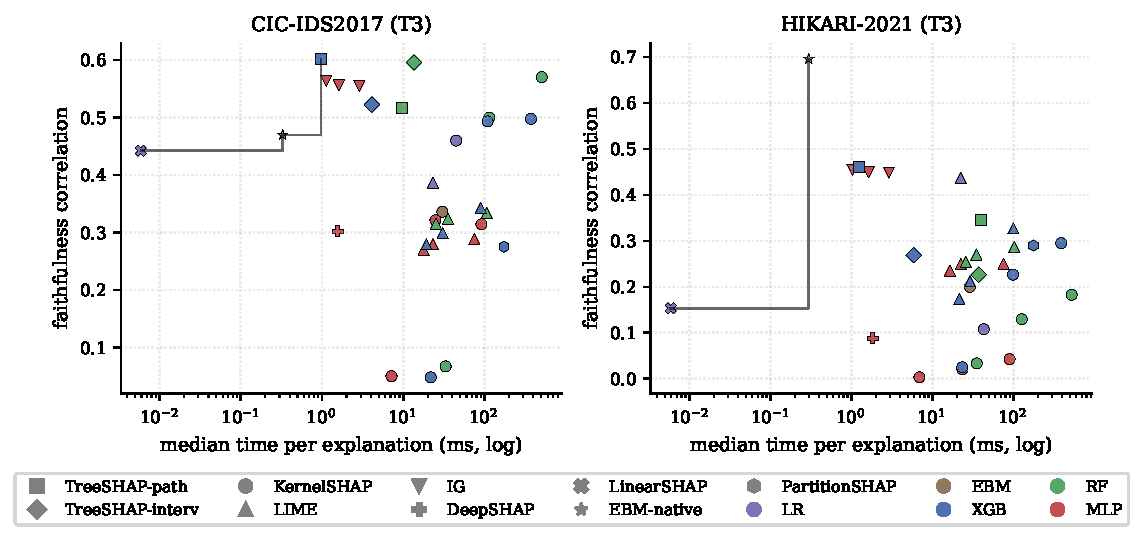
\includegraphics[width=0.9\textwidth]{../figures/fig_cost_fidelity_pareto.pdf}
\caption{Cost versus faithfulness of every explainer on $T_3$. The step line is the best trade-off (cheaper and more faithful is better).}
\label{fig:pareto}
\end{figure}

\subsection{RQ2 --- Are the explanations correct, and does encryption change that?}
\label{sec:rq2}
\begin{itemize}[leftmargin=*, itemsep=0pt]
  \item \textbf{Quality is moderate and depends on the explainer.} Faithfulness is mostly 0.2--0.6 (Table~\ref{tab:costfid}). The best explainer for each detector is a fast one: TreeSHAP for XGBoost (0.60 on CIC-IDS2017, 0.46 on HIKARI), IG for the MLP (0.56 and 0.45), and the EBM's own explanations on HIKARI (0.70). Infidelity and deletion AOPC rank the explainers similarly (Spearman correlation with faithfulness 0.79 and 0.45 on CIC-IDS2017, 0.48 and 0.79 on HIKARI).
  \item \textbf{A bigger budget helps only up to a point.} KernelSHAP with 100 samples is useless (faithfulness about 0), while 500 samples are as good as 2{,}048. More LIME samples or IG steps add little.
  \item \textbf{DeepSHAP is unreliable} for our MLP (faithfulness 0.09--0.30, and unstable on HIKARI).
\end{itemize}

\textbf{Does encryption make explanations worse? Not on CIC-IDS2017.} Hypothesis H2 expected lower quality on $T_3$. Table~\ref{tab:tier} shows the opposite on CIC-IDS2017: faithfulness is significantly \emph{higher} on $T_3$ for 7 of 8 pairs, for example KernelSHAP on XGBoost rises from 0.29 to 0.49. The reason is that with all features, half of XGBoost's explanation weight sits on ports and TCP flags, which are known recording artefacts of this dataset~\cite{engelen2021}. On $T_3$ the weight moves to packet-size statistics, which describe the traffic itself and are easier to explain. On HIKARI the result is mixed: 3 pairs get worse, 1 gets better and 4 do not change. Features do become more correlated on $T_3$, as expected (mean $|\rho_s|$ 0.36 $\rightarrow$ 0.43 on CIC-IDS2017).

\begin{table}[!htbp]
\centering
\caption{Faithfulness with all features ($T_1$) and with the encrypted-traffic view ($T_3$) on the same flows. $p$ = paired Wilcoxon test, Holm-corrected.}
\label{tab:tier}
\scriptsize
\setlength{\tabcolsep}{2.5pt}
\begin{minipage}[t]{0.495\textwidth}
\centering
\begin{tabular}{llrrrr}
\toprule
\multicolumn{6}{c}{\textbf{CIC-IDS2017}} \\
\midrule
\textbf{Model} & \textbf{Explainer} & \textbf{$T_1$} & \textbf{$T_3$} & \textbf{$\Delta$} & \textbf{$p$} \\
\midrule
MLP & DeepSHAP & 0.23 & 0.30 & 0.07 & 7e-04 \\
MLP & IG-32 & 0.47 & 0.56 & 0.09 & 3e-07 \\
MLP & KernelSHAP-500 & 0.29 & 0.32 & 0.03 & 0.22 \\
MLP & LIME-1000 & 0.22 & 0.28 & 0.06 & 4e-03 \\
XGB & KernelSHAP-500 & 0.29 & 0.49 & 0.20 & 2e-14 \\
XGB & LIME-1000 & 0.23 & 0.30 & 0.07 & 2e-04 \\
XGB & TreeSHAP-interv & 0.35 & 0.52 & 0.17 & 1e-14 \\
XGB & TreeSHAP-path & 0.52 & 0.60 & 0.08 & 3e-05 \\
\bottomrule
\end{tabular}
\end{minipage}
\hfill
\begin{minipage}[t]{0.495\textwidth}
\centering
\begin{tabular}{llrrrr}
\toprule
\multicolumn{6}{c}{\textbf{HIKARI-2021}} \\
\midrule
\textbf{Model} & \textbf{Explainer} & \textbf{$T_1$} & \textbf{$T_3$} & \textbf{$\Delta$} & \textbf{$p$} \\
\midrule
MLP & DeepSHAP & 0.10 & 0.09 & -0.02 & 0.69 \\
MLP & IG-32 & 0.49 & 0.45 & -0.04 & 0.69 \\
MLP & KernelSHAP-500 & 0.14 & 0.02 & -0.12 & 9e-13 \\
MLP & LIME-1000 & 0.27 & 0.25 & -0.02 & 0.69 \\
XGB & KernelSHAP-500 & 0.28 & 0.23 & -0.05 & 0.02 \\
XGB & LIME-1000 & 0.16 & 0.21 & 0.05 & 4e-03 \\
XGB & TreeSHAP-interv & 0.35 & 0.27 & -0.08 & 1e-07 \\
XGB & TreeSHAP-path & 0.49 & 0.46 & -0.03 & 0.69 \\
\bottomrule
\end{tabular}
\end{minipage}
\end{table}


\textbf{Explainers disagree.} Two explainers share on average only about 2 of their top-5 features (Jaccard@5 0.19--0.31 for the tree models and the MLP; Fig.~\ref{fig:agreement}). Only two methods that estimate the same quantity agree well (KernelSHAP-2048 and interventional TreeSHAP: 0.71). The explanation an analyst sees therefore depends on the chosen explainer, so its quality has to be measured, not assumed.

\begin{figure}[!htbp]
\centering
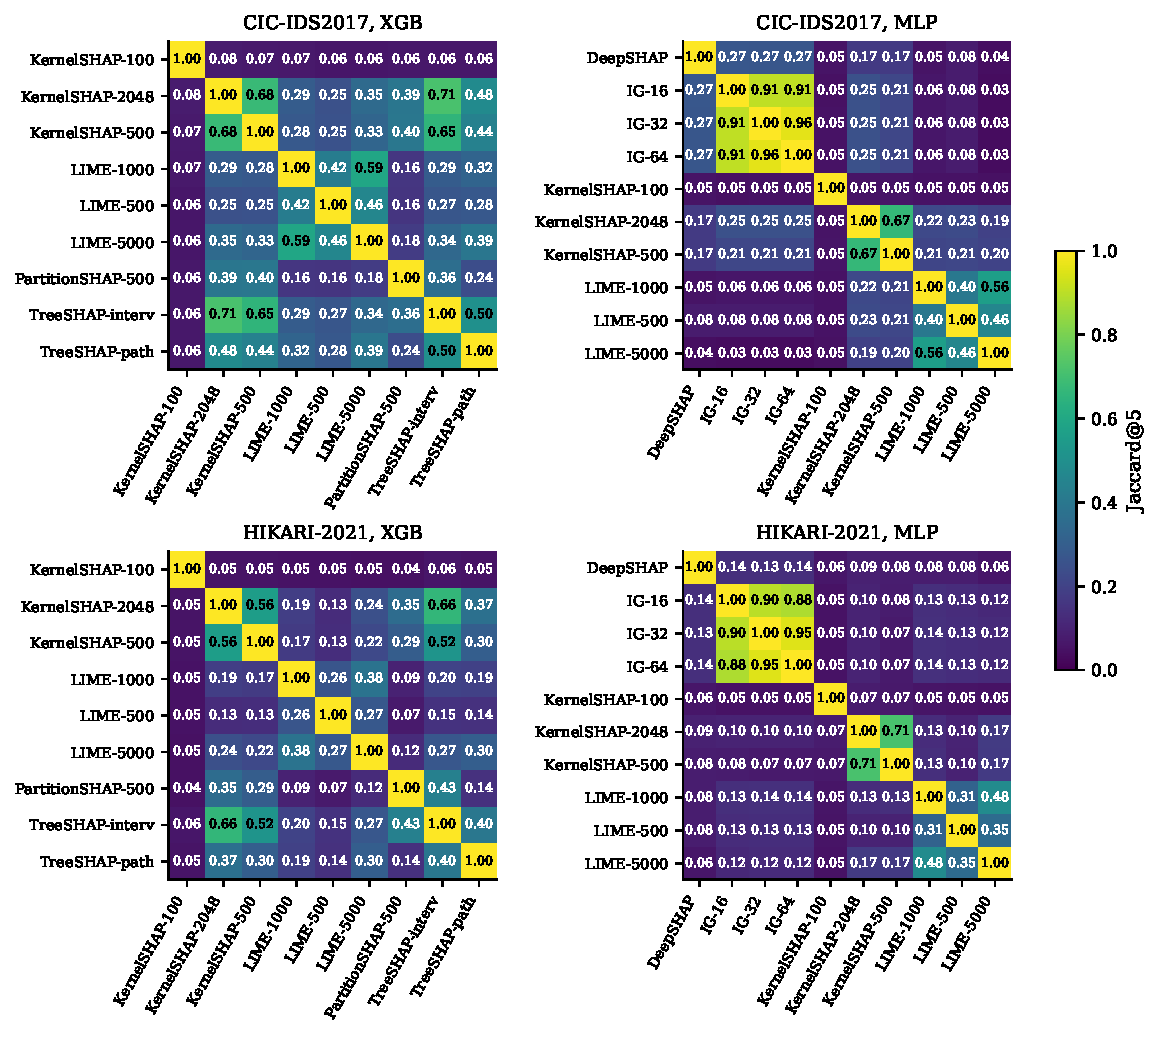
\includegraphics[width=0.72\textwidth]{../figures/fig_agreement.pdf}
\caption{Top-5 agreement (Jaccard@5) between explainers on the same flows ($T_3$).}
\label{fig:agreement}
\end{figure}

\subsection{RQ3 --- Do explanations stay the same when the network changes?}
\label{sec:rq3}
We compared the top-5 features of the four attack families shared by CIC-IDS2017 and CSE-CIC-IDS2018 (Fig.~\ref{fig:drift}).
\begin{itemize}[leftmargin=*, itemsep=0pt]
  \item \textbf{Within one network, explanations are stable:} two random halves of the data agree 0.99 (Jaccard@5), and a model retrained with another seed still agrees 0.82. They also stay stable over time.
  \item \textbf{Across networks they change:} agreement falls to 0.48 when the same model is used on the other network, and to 0.17 when each network has its own model. That is below both noise levels in 12 of 16 cases.
  \item \textbf{The change follows the accuracy loss} (Spearman $\rho=0.63$, $p=0.008$). For DoS, recall falls from 0.94 to 0.43 and top-5 agreement to 0.43, so the model shows confident but outdated reasons for exactly the flows it now misses.
  \item \textbf{Transfer costs 20--34 F1 points.} Hiding ports and headers ($T_3$) lowers the false-positive rate after the change (9.9--11.9\% instead of 16.8--19.4\% on $T_1$).
\end{itemize}
H3 is supported: watching explanation drift can warn of a network change before labelled data are available.

\begin{figure}[!htbp]
\centering
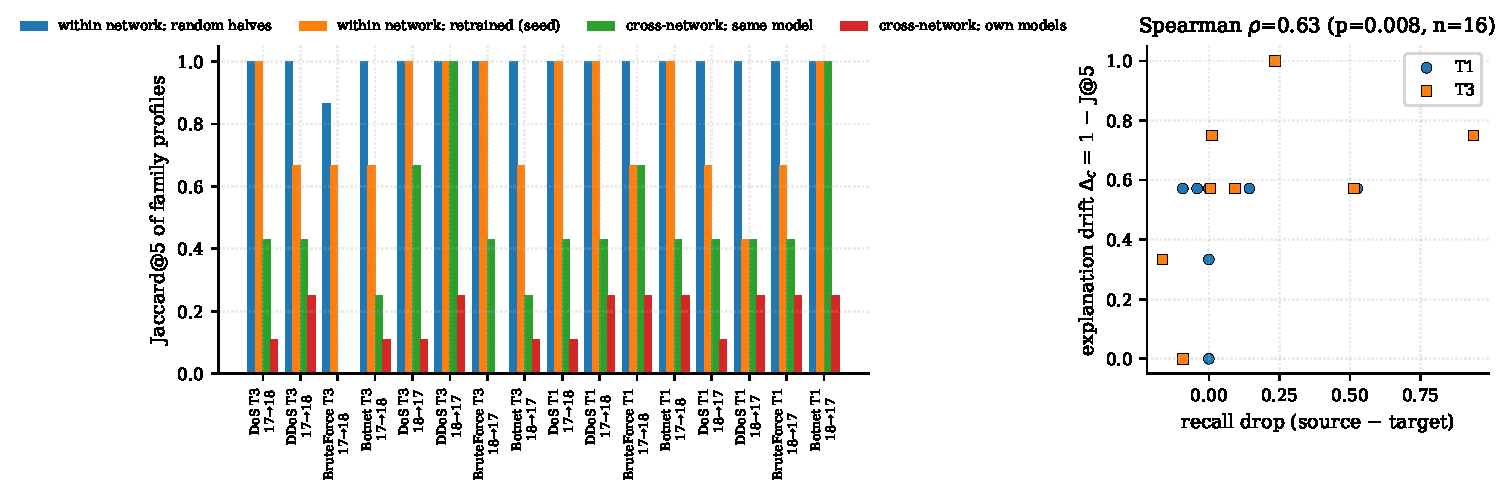
\includegraphics[width=0.9\textwidth]{../figures/fig_drift.pdf}
\caption{Left: top-5 agreement of attack-family explanations within one network (two noise levels) and across networks. Right: explanation drift against the drop in recall for the same family.}
\label{fig:drift}
\end{figure}

\subsection{RQ4 --- Does the selective trigger work under live traffic?}
\label{sec:rq4}
Table~\ref{tab:stream} compares the policies at 75\% load on CIC-IDS2017, and Fig.~\ref{fig:stream:cic} shows all three loads.

\begin{table}[!htbp]
\centering
\caption{Explanation policies on CIC-IDS2017 at 75\% load. Overhead = explanation work as a share of detection time; Covered = share of true alerts with an exact explanation within 1\,s; Delay = 99th-percentile time to a verdict in seconds.}
\label{tab:stream}
\scriptsize
\setlength{\tabcolsep}{4pt}
\begin{minipage}[t]{0.495\textwidth}
\centering
\begin{tabular}{lrrr}
\toprule
\multicolumn{4}{c}{\textbf{Normal (mixed) traffic}} \\
\midrule
\textbf{Policy} & \textbf{Overhead} & \textbf{Covered} & \textbf{Delay (s)} \\
\midrule
B1 explain none & 0.00 & 0.00 & 0.003 \\
B2a all, TreeSHAP & 2.14 & 0.06 & 16.72 \\
B2b all, KernelSHAP & 257.67 & 0.00 & 2117.02 \\
B3 one global expl. & 0.00 & 0.00 & 0.058 \\
B4 random & 0.37 & 0.16 & 0.243 \\
B5 every alert & 0.13 & 1.00 & 0.008 \\
B6 learned explainer & 0.29 & 0.75 & 1.44 \\
\textbf{Proposed} & 0.11 & 1.00 & 0.032 \\
\bottomrule
\end{tabular}
\end{minipage}
\hfill
\begin{minipage}[t]{0.495\textwidth}
\centering
\begin{tabular}{lrrr}
\toprule
\multicolumn{4}{c}{\textbf{With port-scan flood}} \\
\midrule
\textbf{Policy} & \textbf{Overhead} & \textbf{Covered} & \textbf{Delay (s)} \\
\midrule
B1 explain none & 0.00 & 0.00 & 0.006 \\
B2a all, TreeSHAP & 2.15 & 0.01 & 18.68 \\
B2b all, KernelSHAP & 242.34 & 0.00 & 2435.23 \\
B3 one global expl. & 0.00 & 0.00 & 0.004 \\
B4 random & 0.60 & 0.03 & 2.58 \\
B5 every alert & 0.42 & 0.41 & 2.68 \\
B6 learned explainer & 0.29 & 1.00 & 0.670 \\
\textbf{Proposed} & 0.10 & 1.00 & 0.035 \\
\bottomrule
\end{tabular}
\end{minipage}
\end{table}


\begin{itemize}[leftmargin=*, itemsep=0pt]
  \item \textbf{Explaining every flow is impossible.} With TreeSHAP it costs 2.1 times the detection time, so verdicts are delayed by 17--19\,s; with KernelSHAP it costs about 250 times. The learned explainer (B6) is cheaper (0.29) but still delays verdicts by 0.7--1.4\,s, and its explanations differ from exact TreeSHAP.
  \item \textbf{In normal traffic, explaining every alert (B5) is affordable} (overhead 0.13, delay 8\,ms). The trigger also explains every alert within 1\,s (57\% instantly) at overhead 0.106 and a 32\,ms delay. On top of that it explains uncertain flows, which include 20 of the 22 attacks the detector missed.
  \item \textbf{During the flood, only the trigger stays fast.} B5's overhead rises to 0.42 and its delay to 2.7\,s, and only 41\% of alerts are explained in time. The trigger keeps overhead at 0.105 and delay at 35\,ms and explains every alert within 1\,s, because flood flows are near-copies and the cache answers 61\% of requests. Cached explanations are as good as fresh ones (faithfulness 0.563 vs.\ 0.575).
  \item \textbf{At overload (150\%)} no policy keeps up. The trigger pauses explanation and stays at the explain-nothing delay (2.7--3.1\,s).
  \item \textbf{Limit:} one core of KernelSHAP finishes about 9 explanations per second, so on CIC-IDS2017 only 24--26\% of the deep requests finish within 30\,s.
  \item \textbf{HIKARI shows the same pattern:} overhead 0.101--0.102, every alert explained within 1\,s, and a delay of 5--19\,ms, against 318\,ms for B5 during the flood.
\end{itemize}
\textbf{H4 is supported within detection capacity:} the overhead is 0.101--0.106 (the 10\% budget plus a small burst allowance), all true alerts are explained within 1\,s, and the delivered explanations are statistically equivalent in quality to fresh exact ones (TOST, margin 0.05).

\begin{figure}[!htbp]
\centering
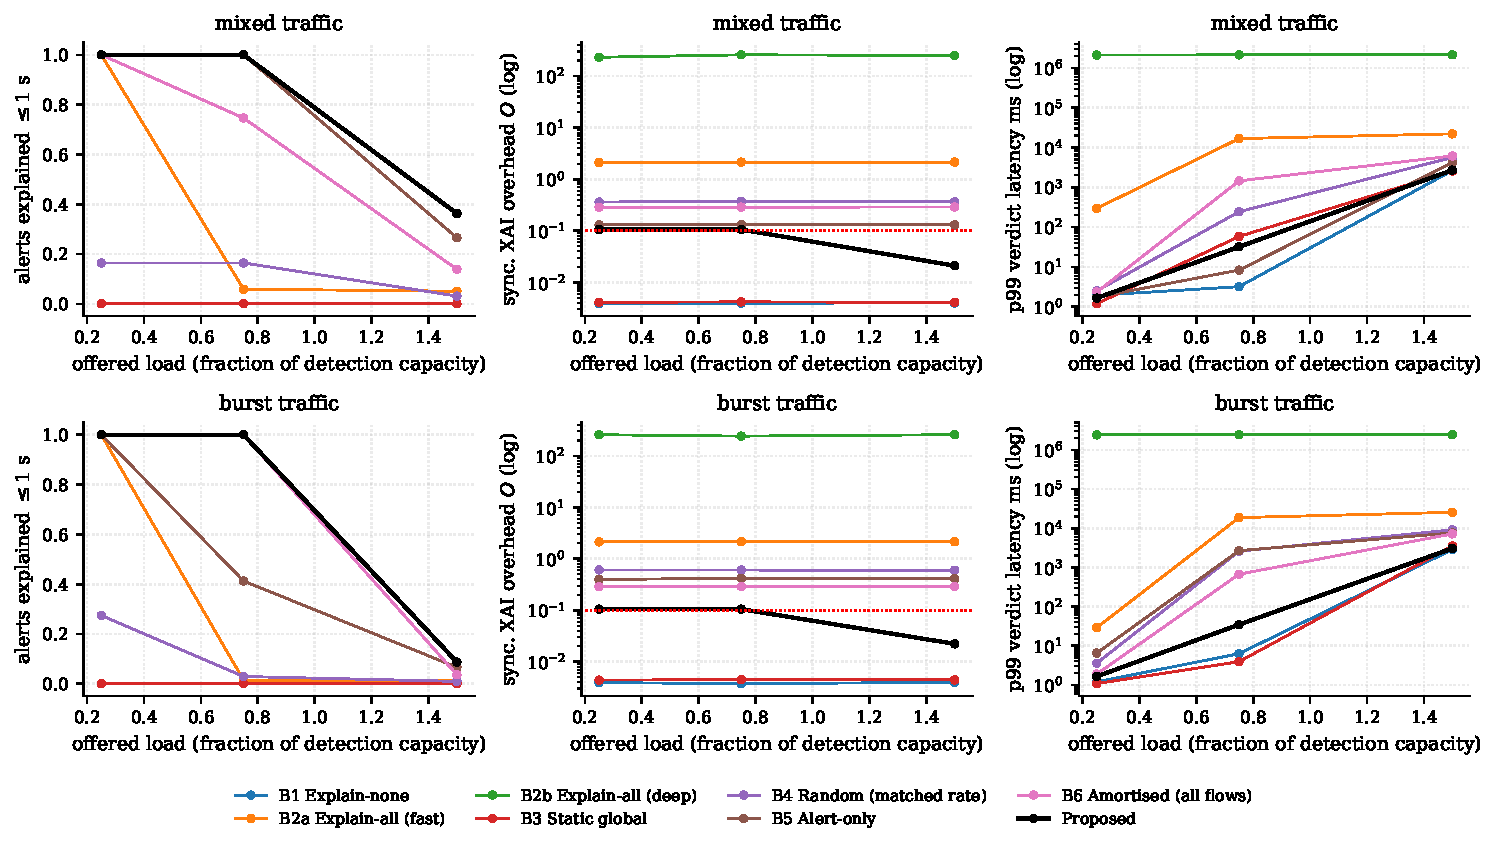
\includegraphics[width=\textwidth]{../figures/fig_stream_cic2017_XGB_T3.pdf}
\caption{CIC-IDS2017, XGBoost on $T_3$: alerts explained within 1\,s (left), explanation overhead (middle; dotted line = 10\% budget) and 99th-percentile verdict delay (right) against load, for normal (top) and flood (bottom) traffic.}
\label{fig:stream:cic}
\end{figure}


% ══════════════════════════════════════════════════════════════════
%  SECTION V --- COMPARISON WITH EXISTING RESEARCH
% ══════════════════════════════════════════════════════════════════
\section{Comparison with Existing Research}
\label{sec:compare}
Where a published study used the same dataset or setup, we place its number next to ours (Table~\ref{tab:compare}). Because hardware and setups differ between studies, we also re-ran the most common published setups on our own data and laptop: TreeSHAP on tree models (P5, P6, P8, P9, P10~\cite{p5,p6,p8,p9,p10}), LIME with 5{,}000 samples (P5), KernelSHAP and DeepSHAP on a neural network (P2~\cite{p2}), and the cross-dataset test of P9. The encrypted-traffic studies we reviewed (P1, P3, P4, P7~\cite{p1,p3,p4,p7}) report neither explanation cost nor quality, so only their detection results can be compared.

\begin{table}[!htbp]
\centering
\caption{Our results next to published results}
\label{tab:compare}
\scriptsize
\setlength{\tabcolsep}{3.5pt}
\begin{tabularx}{\textwidth}{>{\raggedright\arraybackslash}p{2.5cm} >{\raggedright\arraybackslash}p{3.9cm} >{\raggedright\arraybackslash}p{3.9cm} Y}
\toprule
\textbf{Aspect} & \textbf{Published result} & \textbf{This study} & \textbf{Comparable?} \\
\midrule
\multicolumn{4}{l}{\textit{Detection}} \\
CIC-IDS2017, same network & P9: RF macro-F1 0.99 (random split) & RF macro-F1 0.81 (time split); binary F1 0.99 & Partly: our split is stricter \\
CIC-IDS2017 $\rightarrow$ 2018 & P9: RF macro-F1 0.13--0.21 & RF macro-F1 0.22 ($T_1$ and $T_3$) & Yes: same test, same result \\
Cross-network transfer & R3~\cite{cerasuolo2026}: F1 drops 40--80\% & F1 drops 20--35\% & Different data, same trend \\
HIKARI-2021 & Vitorino et al.~\cite{vitorino2024}: F1 83.5--83.7\% (random split) & F1 0.12--0.26 at 1\% FPR; 0.69--0.73 at best threshold & No: leak in the public file (see text) \\
\midrule
\multicolumn{4}{l}{\textit{Explanation cost (per flow)}} \\
TreeSHAP on XGBoost & P5: 20--80\,ms; P6: 30--34\,ms per alert & 0.98\,ms (+30\,ms to build once) & Published times include building \\
LIME, 5{,}000 samples & P5: 4.9--36\,s & 90\,ms & Settings not reported \\
KernelSHAP, neural net & P2: about 9.2\,s & 92\,ms (2{,}048 samples) & Settings not reported \\
DeepSHAP / IG & P2: 132\,ms / 0.09\,ms (batch average) & 1.6\,ms / 1.1\,ms (single flow) & Batch vs.\ single flow \\
Detector time & P8: XGBoost 31\,ms (Raspberry~Pi); P7: microseconds (batch) & XGBoost 0.38--0.55\,ms & Different hardware \\
\midrule
\multicolumn{4}{l}{\textit{Explanation policy and quality}} \\
When to explain & R2~\cite{dmthreatnet2026}: never per flow; P8: every alert & Trigger: overhead 0.10, all alerts within 1\,s, flood delay 5--35\,ms & First measured policy \\
Stability across seeds & P10: 0.86--0.90 & 0.82 (Jaccard@5) & Different index, similar level \\
SHAP vs.\ LIME agreement & P5: $\kappa = 0.94$ (unencrypted data) & Jaccard@5 0.30--0.39 & Much lower on metadata \\
\bottomrule
\end{tabularx}
\end{table}

\begin{itemize}[leftmargin=*, itemsep=0pt]
  \item \textbf{Detection matches when the setup matches.} Like P9, our Random Forest collapses when moved from CIC-IDS2017 to CIC-IDS2018 (macro-F1 0.22 vs.\ 0.13--0.21). Our same-network score is lower than P9's (0.81 vs.\ 0.99) because we split by time and remove duplicates; a random split puts near-copies of test flows into training~\cite{arp2022}.
  \item \textbf{HIKARI's published 83\% F1 could not be reproduced.} The public HIKARI file is sorted by traffic type and contains two row-number columns; one of them alone separates attacks from normal traffic with ROC-AUC 0.93. This is a data leak, and we remove both columns.
  \item \textbf{Published SHAP costs look high because of what was timed.} Building a TreeSHAP explainer takes 30\,ms, but explaining one flow takes only 0.98\,ms; P6's 30--34\,ms per alert matches the sum. Batch averages (P2) hide the real per-flow cost in the other direction, and R1~\cite{kalakoti2026} calls SHAP and LIME ``heavy'' without giving numbers.
  \item \textbf{Explainers agree much less on encrypted metadata} than on unencrypted data (TreeSHAP vs.\ LIME share 2--3 of their top-5 features, against $\kappa=0.94$ in P5).
\end{itemize}
\textbf{Limits of the comparison.} Studies use different hardware, time different things (one flow, one alert or a batch), use different dataset versions and splits and different quality metrics, and often do not report key settings. All our numerical claims therefore rest on our own re-runs; published numbers only show where our results sit.

% ══════════════════════════════════════════════════════════════════
%  SECTION VI --- ABLATION STUDIES
% ══════════════════════════════════════════════════════════════════
\section{Ablation Studies}
\label{sec:ablation}
All ablations planned in Phase~2 were run except A9, which needs packet sequences. A7, the visibility tier, is covered throughout Section~\ref{sec:results}.

\subsection{Parts of the trigger (A1--A6)}
\label{sec:abl:trigger}
Each variant removes or changes one part of the trigger and is replayed on exactly the same traffic as in Section~\ref{sec:rq4} (Table~\ref{tab:abl}).

\begin{table}[!htbp]
\centering
\caption{Trigger ablations on CIC-IDS2017 at 75\% load (each row removes or changes one part). Instant = share of alerts explained on the detection path within 1\,s; Deep = share of KernelSHAP requests finished within 30\,s; Delay in ms.}
\label{tab:abl}
\scriptsize
\setlength{\tabcolsep}{3pt}
\begin{minipage}[t]{0.495\textwidth}
\centering
\begin{tabular}{lrrrr}
\toprule
\multicolumn{5}{c}{\textbf{Normal (mixed) traffic}} \\
\midrule
\textbf{Variant} & \textbf{Overhead} & \textbf{Instant} & \textbf{Deep} & \textbf{Delay} \\
\midrule
\textbf{Full trigger} & 0.11 & 0.57 & 0.24 & 32 \\
A1 no uncertainty rule & 0.11 & 0.86 & 1.00 & 12 \\
A2 no novelty rule & 0.11 & 0.73 & 0.25 & 36 \\
A3 no cache & 0.11 & 0.15 & 0.16 & 38 \\
A4 no budget limit & 0.24 & 1.00 & 0.26 & 100 \\
A5a no deep lane & 0.11 & 0.60 & -- & 18 \\
A5b KernelSHAP only & 0.05 & 0.00 & 0.18 & 12 \\
A6 budget 2\% & 0.06 & 0.19 & 0.24 & 11 \\
A6 budget 5\% & 0.06 & 0.21 & 0.24 & 12 \\
A6 budget 20\% & 0.20 & 0.91 & 0.24 & 108 \\
\bottomrule
\end{tabular}
\end{minipage}
\hfill
\begin{minipage}[t]{0.495\textwidth}
\centering
\begin{tabular}{lrrrr}
\toprule
\multicolumn{5}{c}{\textbf{With port-scan flood}} \\
\midrule
\textbf{Variant} & \textbf{Overhead} & \textbf{Instant} & \textbf{Deep} & \textbf{Delay} \\
\midrule
\textbf{Full trigger} & 0.10 & 0.88 & 0.26 & 35 \\
A1 no uncertainty rule & 0.10 & 0.96 & 1.00 & 58 \\
A2 no novelty rule & 0.09 & 0.92 & 0.25 & 151 \\
A3 no cache & 0.11 & 0.05 & 0.15 & 18 \\
A4 no budget limit & 0.23 & 1.00 & 0.26 & 113 \\
A5a no deep lane & 0.10 & 0.85 & -- & 23 \\
A5b KernelSHAP only & 0.06 & 0.00 & 0.18 & 6 \\
A6 budget 2\% & 0.06 & 0.31 & 0.25 & 62 \\
A6 budget 5\% & 0.06 & 0.31 & 0.24 & 26 \\
A6 budget 20\% & 0.20 & 0.98 & 0.27 & 31 \\
\bottomrule
\end{tabular}
\end{minipage}
\end{table}


\begin{itemize}[leftmargin=*, itemsep=0pt]
  \item \textbf{A1, uncertainty rule:} removing it frees budget (57\% $\rightarrow$ 86\% of alerts explained instantly), but then none of the 20 missed attacks is explained. It is the only part that shows analysts the detector's mistakes.
  \item \textbf{A2, novelty rule:} the most expensive part (it raises the trigger's own cost from 1\% to 5\% of detection time). It only pays off when the network changes (RQ3).
  \item \textbf{A3, cache:} without it, instant coverage falls to 15\% in normal traffic and 5\% during the flood.
  \item \textbf{A4, budget limit:} without it, overhead jumps to 0.23--0.24 and the delay triples (100--113\,ms).
  \item \textbf{A5, two lanes:} running KernelSHAP on the detection path (A5b) explains no alert in time. The fast lane gives coverage; the deep lane adds KernelSHAP only within its capacity.
  \item \textbf{A6, budget size:} overhead follows the budget (0.20 at a 20\% budget) but cannot go below about 0.05, the trigger's own cost. A narrower uncertainty band (2\% instead of 5\%) raises deep coverage from 24\% to 58\%.
\end{itemize}

\subsection{Features and explainer (A8, A10, A11)}
\label{sec:abl:repr}
\begin{table}[!htbp]
\centering
\caption{Ablations of the features and the explainer (XGBoost, $T_3$, 100 flows): A8 trains on one feature group, A10 explains groups of related features, A11 changes the KernelSHAP background size.}
\label{tab:extra}
\scriptsize
\setlength{\tabcolsep}{4pt}
\begin{minipage}[t]{0.495\textwidth}
\centering
\begin{tabular}{lrrr}
\toprule
\multicolumn{4}{c}{\textbf{CIC-IDS2017}} \\
\midrule
\textbf{Variant} & \textbf{F1} & \textbf{Faith.} & \textbf{ms} \\
\midrule
A8 timing only & 0.913 & 0.35 & 6.2 \\
A8 sizes only & 0.668 & 0.37 & 3.7 \\
A8 volume/direction only & 0.767 & 0.27 & 6.5 \\
A8 all $T_3$ features & 0.984 & 0.49 & 4.4 \\
A11 background 10 & -- & 0.36 & 26.3 \\
A11 background 50 & -- & 0.51 & 94.2 \\
A11 background 100 & -- & 0.50 & 173.8 \\
A10 per feature (KernelSHAP) & -- & 0.49 & 94.8 \\
A10 grouped (PartitionSHAP) & -- & 0.30 & 158.1 \\
\bottomrule
\end{tabular}
\end{minipage}
\hfill
\begin{minipage}[t]{0.495\textwidth}
\centering
\begin{tabular}{lrrr}
\toprule
\multicolumn{4}{c}{\textbf{HIKARI-2021}} \\
\midrule
\textbf{Variant} & \textbf{F1} & \textbf{Faith.} & \textbf{ms} \\
\midrule
A8 timing only & 0.248 & 0.06 & 7.2 \\
A8 sizes only & 0.114 & 0.14 & 6.1 \\
A8 volume/direction only & 0.096 & -0.00 & 5.7 \\
A8 all $T_3$ features & 0.262 & 0.27 & 5.8 \\
A11 background 10 & -- & 0.25 & 28.0 \\
A11 background 50 & -- & 0.25 & 93.0 \\
A11 background 100 & -- & 0.23 & 178.5 \\
A10 per feature (KernelSHAP) & -- & 0.24 & 91.3 \\
A10 grouped (PartitionSHAP) & -- & 0.30 & 160.2 \\
\bottomrule
\end{tabular}
\end{minipage}
\end{table}


\begin{itemize}[leftmargin=*, itemsep=0pt]
  \item \textbf{A8, feature groups:} on CIC-IDS2017, timing features alone reach F1 0.913 against 0.984 with all features, and explanations are best with all features. On HIKARI, timing alone detects almost as well as all features (F1 0.248 vs.\ 0.262), but its explanations are nearly meaningless (0.055). Good detection does not guarantee a trustworthy explanation.
  \item \textbf{A10, grouped explanations:} PartitionSHAP is worse than KernelSHAP on CIC-IDS2017 (0.30 vs.\ 0.49), better on HIKARI (0.30 vs.\ 0.24), and costs 1.7 times more. Grouping is not a general fix.
  \item \textbf{A11, background size:} 10 background points cut KernelSHAP's cost to 26--28\,ms but lose a third of its faithfulness on CIC-IDS2017; 100 points double the cost with no gain. 50 points is the best trade-off.
\end{itemize}

\subsection{Known-answer check of the explainers}
\label{sec:abl:sanity}
Faithfulness scores (RQ2) have no ground truth, so we also ran a test where the correct answer is known. A random feature was added to the CIC-IDS2017 $T_3$ data, and every benign flow with a high value of it was relabelled as an attack. After retraining, this planted feature is the true reason for those alerts and irrelevant for real attacks (Table~\ref{tab:sanity}).

\begin{table}[!htbp]
\centering
\caption{Known-answer test (CIC-IDS2017, $T_3$). Found = share of the 100 flows that are attacks only because of the planted feature where it is ranked first (should be 1); Weight = its share of the explanation for those flows; Wrong = share of 100 real attacks where the irrelevant planted feature is ranked first (should be 0).}
\label{tab:sanity}
\scriptsize
\setlength{\tabcolsep}{5pt}
\begin{minipage}[t]{0.495\textwidth}
\centering
\begin{tabular}{lrrr}
\toprule
\multicolumn{4}{c}{\textbf{XGBoost}} \\
\midrule
\textbf{Explainer} & \textbf{Found} & \textbf{Weight} & \textbf{Wrong} \\
\midrule
TreeSHAP-path & 1.00 & 0.66 & 0.01 \\
TreeSHAP-interv & 1.00 & 0.75 & 0.00 \\
KernelSHAP-100 & 0.85 & 0.30 & 0.02 \\
KernelSHAP-500 & 1.00 & 0.79 & 0.00 \\
LIME-1000 & 1.00 & 0.27 & 0.88 \\
PartitionSHAP-500 & 1.00 & 0.88 & 0.00 \\
\bottomrule
\end{tabular}
\end{minipage}
\hfill
\begin{minipage}[t]{0.495\textwidth}
\centering
\begin{tabular}{lrrr}
\toprule
\multicolumn{4}{c}{\textbf{MLP}} \\
\midrule
\textbf{Explainer} & \textbf{Found} & \textbf{Weight} & \textbf{Wrong} \\
\midrule
IG-16 & 0.99 & 0.58 & 0.16 \\
DeepSHAP & 0.00 & 0.03 & 0.00 \\
KernelSHAP-100 & 0.47 & 0.08 & 0.01 \\
KernelSHAP-500 & 1.00 & 0.37 & 0.05 \\
LIME-1000 & 1.00 & 0.17 & 0.55 \\
\bottomrule
\end{tabular}
\end{minipage}
\end{table}


\begin{itemize}[leftmargin=*, itemsep=0pt]
  \item \textbf{The detectors really use the planted feature:} XGBoost flags 100\% of the planted attacks and the MLP 84\%.
  \item \textbf{TreeSHAP, KernelSHAP-500 and PartitionSHAP pass:} they rank the planted feature first for every planted attack and almost never for real attacks (0--1\% on XGBoost). IG also finds it (99\%) but wrongly ranks it first for 16\% of real attacks.
  \item \textbf{LIME finds it but also blames it when it played no role} (88\% of real attacks on XGBoost, 55\% on the MLP), because it samples far away from the explained flow.
  \item \textbf{DeepSHAP never finds it} (0\%) and KernelSHAP-100 often misses it (85\% and 47\%), which matches the RQ2 finding that both are unreliable.
\end{itemize}

\subsection{Robustness and repeatability}
\label{sec:abl:robust}
\begin{itemize}[leftmargin=*, itemsep=0pt]
  \item \textbf{CIC-IDS2017 is robust} (Fig.~\ref{fig:robust}): with timing changed by up to $\pm$50\% or sizes padded by up to 50\%, F1 stays at 0.981--0.984 for XGBoost and 0.961--0.970 for the MLP, and top-5 explanations change only slowly (Jaccard@5 0.85--0.91 at 50\%).
  \item \textbf{HIKARI XGBoost is fragile to padding:} just 5\% size padding cuts its F1 from 0.262 to 0.078. TLS~1.3 and QUIC allow padding, so padding tests should be part of every encrypted-traffic IDS evaluation.
  \item \textbf{Timing is repeatable:} repeating eight settings three times varied by 1.0--13.5\%, far less than the 5--1{,}000$\times$ differences between explainers.
\end{itemize}
Every number and table in this report is produced by scripts from the saved results (\texttt{code/README.md}).

\begin{figure}[!htbp]
\centering
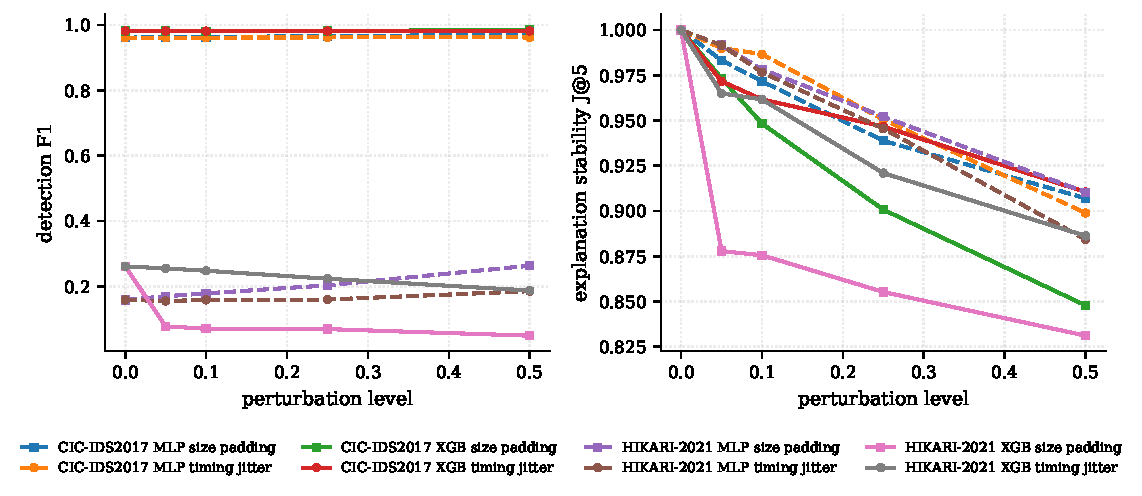
\includegraphics[width=0.62\textwidth]{../figures/fig_robustness.pdf}
\caption{Detection F1 (left) and top-5 explanation stability (right) under increasing timing jitter and size padding.}
\label{fig:robust}
\end{figure}

% ══════════════════════════════════════════════════════════════════
%  SECTION VII --- RESULTS ANALYSIS AND DISCUSSION
% ══════════════════════════════════════════════════════════════════
\section{Results Analysis and Discussion}
\label{sec:discussion}

\subsection{Hypotheses}
\begin{table}[H]
\centering
\caption{Verdicts on the Phase 2 hypotheses}
\label{tab:verdicts}
\scriptsize
\setlength{\tabcolsep}{3.5pt}
\begin{tabularx}{\textwidth}{>{\raggedright\arraybackslash}p{4.3cm} Y >{\raggedright\arraybackslash}p{2.4cm}}
\toprule
\textbf{Hypothesis} & \textbf{Evidence} & \textbf{Verdict} \\
\midrule
H1: slow explainers make each flow at least 100$\times$ slower & True for 25 of 44 slow settings (up to 1{,}500$\times$); not on the slow Random Forest or with small budgets; fast explainers add only 1.1--49$\times$ & Partly supported \\
H2: explanation quality falls under encryption & CIC-IDS2017: quality \emph{rises} for 7 of 8 pairs; HIKARI: 3 worse, 1 better, 4 unchanged & Rejected on CIC-IDS2017; mixed on HIKARI \\
H3: explanations change across networks, in step with accuracy loss & Below the noise levels in 12 of 16 cases; drift follows the recall drop ($\rho=0.63$) & Supported \\
H4: the trigger keeps overhead $\le$ 10\%, explains $\ge$ 95\% of alerts in time, with no loss of quality & Overhead 0.101--0.106, 100\% of alerts explained within 1\,s, quality equivalent to fresh explanations & Supported within detection capacity \\
\bottomrule
\end{tabularx}
\end{table}

\subsection{Main findings}
\begin{enumerate}[leftmargin=*, itemsep=0pt]
  \item \textbf{Cost depends on the explainer--detector pair, not on ``XAI'' in general.} Fast model-specific explainers cost about as much as detection and are also the most faithful. XGBoost with TreeSHAP, or an EBM, detects and explains a flow for 1.8--4.2 times the cost of detection alone. KernelSHAP and LIME belong only on a background lane.
  \item \textbf{Encryption removes artefacts, not explainability.} On CIC-IDS2017 the $T_3$ view loses at most 1.5 F1 points, gives more faithful explanations, and produces fewer false positives after a network change.
  \item \textbf{The choice of explainer changes the story.} Explainers share only about 2 of their top-5 features, so a security team should fix one explainer and measure its quality on its own traffic.
  \item \textbf{Explanation drift is a free early warning} of a network change.
  \item \textbf{Selective explanation helps most at the edges:} during floods (cache), under overload (pausing) and for missed attacks (uncertainty rule).
  \item \textbf{Padding is a cheap way to evade} a metadata-based detector, so it should be tested.
\end{enumerate}

\subsection{Research gaps}
Gaps G1--G3 were found in Phase~1 and G4 was added in Phase~2. Table~\ref{tab:gapmap} maps each gap to what this phase shows and what remains open.

\begin{table}[!htbp]
\centering
\caption{Research gaps of Phase 2: what Phase 3 shows and what remains open}
\label{tab:gapmap}
\scriptsize
\setlength{\tabcolsep}{3.5pt}
\begin{tabularx}{\textwidth}{>{\raggedright\arraybackslash}p{3.2cm} Y >{\raggedright\arraybackslash}p{3.8cm}}
\toprule
\textbf{Gap} & \textbf{What Phase 3 shows} & \textbf{Still open} \\
\midrule
G1: explanation cost not measured & Time and memory of every explainer on one core; published costs include explainer building (Sections~\ref{sec:rq1}, \ref{sec:compare}) & Edge devices; GPU batching \\
G2: quality under encryption unknown & Quality of nine explainers on three visibility tiers, with paired tests (Section~\ref{sec:rq2}) & Real QUIC captures; packet-sequence models \\
G3: consistency under network change & Drift beyond the noise levels, linked to accuracy loss (Section~\ref{sec:rq3}) & Other shifts (DoH tunnel tools); drift-triggered retraining \\
G4: no budget-aware explanation policy & A trigger tested against seven baselines and fifteen ablation variants (Sections~\ref{sec:rq4}, \ref{sec:ablation}) & Adaptive budgets; a study with real analysts \\
\bottomrule
\end{tabularx}
\end{table}

\subsection{Strengths and limitations}
\textbf{Strengths.} Cost, quality and drift are measured on the same explanations of the same flows; the data are leakage-controlled with time-based splits; the encryption assumption is tested on real packets; the explainers are checked against a known answer; every comparison uses paired statistical tests with effect sizes; and every result can be regenerated from the code.

\textbf{Limitations.}
\begin{itemize}[leftmargin=*, itemsep=0pt]
  \item The QUIC view is emulated by removing columns from flow datasets, not measured on real QUIC traffic, and the only truly encrypted dataset (HIKARI) has weak detectors.
  \item All timings come from one laptop, with 200 flows per setting and one seed.
  \item Removal-based quality metrics depend on the value that replaces a removed feature; two different replacement values and a known-answer test (Section~\ref{sec:abl:sanity}) gave the same explainer ranking.
  \item Many statistical tests were run, so all of them are Holm-corrected.
\end{itemize}


\FloatBarrier
% ══════════════════════════════════════════════════════════════════
%  REFERENCES (numbered in order of first citation by the cite package)
% ══════════════════════════════════════════════════════════════════
\section*{References}
\begin{multicols}{2}
\renewcommand{\section}[2]{}% the heading is printed above, across both columns
\begin{thebibliography}{99}
\footnotesize

% ---- Phase 1 corpus ----
\bibitem{kalakoti2026}
R.~Kalakoti, H.~Bahsi, and S.~N\~{o}mm, ``Synthetic data-driven explainability for federated learning-based intrusion detection system,'' \textit{IEEE Internet of Things Journal}, vol.~13, no.~4, pp.~5918--5944, Feb. 2026, doi: 10.1109/JIOT.2025.3633946.

\bibitem{dmthreatnet2026}
S.~V. Easwaramoorthy, M.~Bouakkaz, and R.~Somula, ``DMThreatNet: A hybrid data mining framework for early cybersecurity threat detection using ensemble intelligence,'' \textit{Journal of King Saud University -- Computer and Information Sciences}, vol.~38, Art.~no.~509, 2026, doi: 10.1007/s44443-026-00916-y.

\bibitem{cerasuolo2026}
F.~Cerasuolo, G.~Bovenzi, and A.~Pescap\`{e}, ``Cross-network transferability of AI-based network intrusion detection systems in heterogeneous Internet of Things environments,'' \textit{Computer Networks}, vol.~286, Art.~no.~112434, 2026, doi: 10.1016/j.comnet.2026.112434.

% ---- Phase 2 corpus ----
\bibitem{p1}
Z.~Liu, Q.~Wei, Q.~Song, and C.~Duan, ``Fine-grained encrypted traffic classification using dual embedding and graph neural networks,'' \textit{Electronics}, vol.~14, no.~4, Art.~no.~778, 2025, doi: 10.3390/electronics14040778.

\bibitem{p2}
O.~Arreche and M.~Abdallah, ``A comparative analysis of DNN-based white-box explainable AI methods in network security,'' \textit{EURASIP Journal on Information Security}, vol.~2025, Art.~no.~16, 2025, doi: 10.1186/s13635-025-00201-x.

\bibitem{p3}
D.~Di~Monda, A.~Nascita, R.~Carillo, and A.~Pescap\`{e}, ``Analyzing the impact of encryption on traffic classification through explainable AI,'' in \textit{Proc. IFIP Networking Conference}, Limassol, Cyprus, May 2025, pp.~134--139.

\bibitem{p4}
M.~Ghaleb, M.~Hamdan, A.~Y. Barnawi, M.~Gambo, A.~Danasabe, S.~Bello, and A.~Habib, ``Explainable AI for lightweight network traffic classification using depthwise separable convolutions,'' \textit{IEEE Open Journal of the Computer Society}, vol.~6, pp.~908--920, 2025, doi: 10.1109/OJCS.2025.3576495.

\bibitem{p5}
B.~Nugraha, A.~V. Jnanashree, and T.~Bauschert, ``A versatile XAI-based framework for efficient and explainable intrusion detection systems,'' \textit{Annals of Telecommunications}, vol.~80, no.~11, pp.~1095--1120, 2025, doi: 10.1007/s12243-025-01118-9.

\bibitem{p6}
F.~Uccello and S.~Nadjm-Tehrani, ``Feature attribution in 5G intrusion detection: A statistical vs.\ logic-based comparison,'' \textit{Journal of Information Security and Applications}, vol.~99, Art.~no.~104448, 2026, doi: 10.1016/j.jisa.2026.104448.

\bibitem{p7}
M.~Moure-Garrido, C.~Garcia-Rubio, and C.~Campo, ``Unveiling hidden patterns: Self-similarity and entropy for robust encrypted DNS traffic security,'' \textit{Journal of Network and Systems Management}, vol.~34, no.~3, Art.~no.~90, 2026, doi: 10.1007/s10922-026-10069-y.

\bibitem{p8}
Q.~Zeng, M.~Yang, and Y.~Hara, ``Resilient and interpretable power fingerprinting for IoT DDoS defense,'' \textit{IEEE Open Journal of the Communications Society}, vol.~7, pp.~4574--4589, 2026, doi: 10.1109/OJCOMS.2026.3690041.

\bibitem{p9}
C.~K{\i}l{\i}\c{c} and G.~\c{S}eng\"{u}l, ``SHAP-guided feature selection for cross-dataset generalization in network intrusion detection systems,'' \textit{IEEE Access}, vol.~14, pp.~90926--90936, 2026, doi: 10.1109/ACCESS.2026.3703481.

\bibitem{p10}
E.~M. Maseno, Y.~Sun, and Z.~Wang, ``Reliability auditing of explanations for machine-learning-based intrusion detection systems,'' \textit{Journal of Computer Virology and Hacking Techniques}, vol.~22, Art.~no.~80, 2026, doi: 10.1007/s11416-026-00664-7.

% ---- Standards ----
\bibitem{rfc9000}
J.~Iyengar and M.~Thomson, ``QUIC: A UDP-Based Multiplexed and Secure Transport,'' IETF RFC~9000, May 2021.

% ---- Explainers and explanation evaluation ----
\bibitem{lundberg2017}
S.~M. Lundberg and S.-I. Lee, ``A unified approach to interpreting model predictions,'' in \textit{Proc. 31st Conf. Neural Information Processing Systems (NeurIPS)}, 2017, pp.~4765--4774.

\bibitem{lundberg2020}
S.~M. Lundberg, G.~Erion, H.~Chen, A.~DeGrave, J.~M. Prutkin, B.~Nair, R.~Katz, J.~Himmelfarb, N.~Bansal, and S.-I. Lee, ``From local explanations to global understanding with explainable AI for trees,'' \textit{Nature Machine Intelligence}, vol.~2, pp.~56--67, 2020.

\bibitem{ribeiro2016}
M.~T. Ribeiro, S.~Singh, and C.~Guestrin, ```Why should I trust you?': Explaining the predictions of any classifier,'' in \textit{Proc. 22nd ACM SIGKDD Int. Conf. Knowledge Discovery and Data Mining}, 2016, pp.~1135--1144.

\bibitem{sundararajan2017}
M.~Sundararajan, A.~Taly, and Q.~Yan, ``Axiomatic attribution for deep networks,'' in \textit{Proc. 34th Int. Conf. Machine Learning (ICML)}, 2017, pp.~3319--3328.

\bibitem{shrikumar2017}
A.~Shrikumar, P.~Greenside, and A.~Kundaje, ``Learning important features through propagating activation differences,'' in \textit{Proc. 34th Int. Conf. Machine Learning (ICML)}, 2017, pp.~3145--3153.

\bibitem{fastshap}
N.~Jethani, M.~Sudarshan, I.~Covert, S.-I. Lee, and R.~Ranganath, ``FastSHAP: Real-time Shapley value estimation,'' in \textit{Proc. Int. Conf. Learning Representations (ICLR)}, 2022.

\bibitem{bhatt2020}
U.~Bhatt, A.~Weller, and J.~M.~F. Moura, ``Evaluating and aggregating feature-based model explanations,'' in \textit{Proc. 29th Int. Joint Conf. Artificial Intelligence (IJCAI)}, 2020, pp.~3016--3022.

\bibitem{samek2017}
W.~Samek, A.~Binder, G.~Montavon, S.~Lapuschkin, and K.-R. M\"{u}ller, ``Evaluating the visualization of what a deep neural network has learned,'' \textit{IEEE Trans. Neural Networks and Learning Systems}, vol.~28, no.~11, pp.~2660--2673, 2017.

\bibitem{yeh2019}
C.-K. Yeh, C.-Y. Hsieh, A.~S. Suggala, D.~I. Inouye, and P.~Ravikumar, ``On the (in)fidelity and sensitivity of explanations,'' in \textit{Proc. 33rd Conf. Neural Information Processing Systems (NeurIPS)}, 2019.

\bibitem{nori2019}
H.~Nori, S.~Jenkins, P.~Koch, and R.~Caruana, ``InterpretML: A unified framework for machine learning interpretability,'' arXiv:1909.09223, 2019.

\bibitem{rudin2019}
C.~Rudin, ``Stop explaining black box machine learning models for high stakes decisions and use interpretable models instead,'' \textit{Nature Machine Intelligence}, vol.~1, pp.~206--215, 2019.

% ---- Methodology, datasets and tools ----
\bibitem{arp2022}
D.~Arp, E.~Quiring, F.~Pendlebury, A.~Warnecke, F.~Pierazzi, C.~Wressnegger, L.~Cavallaro, and K.~Rieck, ``Dos and don'ts of machine learning in computer security,'' in \textit{Proc. 31st USENIX Security Symposium}, 2022, pp.~3971--3988.

\bibitem{demsar2006}
J.~Dem\v{s}ar, ``Statistical comparisons of classifiers over multiple data sets,'' \textit{Journal of Machine Learning Research}, vol.~7, pp.~1--30, 2006.

\bibitem{ledoit2004}
O.~Ledoit and M.~Wolf, ``A well-conditioned estimator for large-dimensional covariance matrices,'' \textit{Journal of Multivariate Analysis}, vol.~88, no.~2, pp.~365--411, 2004.

\bibitem{chen2016}
T.~Chen and C.~Guestrin, ``XGBoost: A scalable tree boosting system,'' in \textit{Proc. 22nd ACM SIGKDD Int. Conf. Knowledge Discovery and Data Mining}, 2016, pp.~785--794.

\bibitem{hikari}
A.~Ferriyan, A.~H. Thamrin, K.~Takeda, and J.~Murai, ``Generating network intrusion detection dataset based on real and encrypted synthetic attack traffic,'' \textit{Applied Sciences}, vol.~11, no.~17, Art.~no.~7868, 2021.

\bibitem{cicids2017}
I.~Sharafaldin, A.~H. Lashkari, and A.~A. Ghorbani, ``Toward generating a new intrusion detection dataset and intrusion traffic characterization,'' in \textit{Proc. 4th Int. Conf. Information Systems Security and Privacy (ICISSP)}, 2018, pp.~108--116.

\bibitem{engelen2021}
G.~Engelen, V.~Rimmer, and W.~Joosen, ``Troubleshooting an intrusion detection dataset: The CICIDS2017 case study,'' in \textit{Proc. IEEE Security and Privacy Workshops (SPW)}, 2021, pp.~7--12.

\bibitem{liu2022error}
L.~Liu, G.~Engelen, T.~Lynar, D.~Essam, and W.~Joosen, ``Error prevalence in NIDS datasets: A case study on CIC-IDS-2017 and CSE-CIC-IDS-2018,'' in \textit{Proc. IEEE Conf. Communications and Network Security (CNS)}, 2022, pp.~254--262.

\bibitem{vitorino2024}
J.~Vitorino, M.~Silva, E.~Maia, and I.~Pra\c{c}a, ``An adversarial robustness benchmark for enterprise network intrusion detection,'' in \textit{Foundations and Practice of Security (FPS 2023)}, Springer, 2024, doi: 10.1007/978-3-031-57537-2\_1.

\bibitem{nfstream}
Z.~Aouini and A.~Pekar, ``NFStream: A flexible network data analysis framework,'' \textit{Computer Networks}, vol.~204, Art.~no.~108719, 2022.

\end{thebibliography}
\end{multicols}


\end{document}
